\documentclass[12pt,pdf,hyperref={unicode}]{beamer}
%\usetheme{boxes}
\beamertemplatenavigationsymbolsempty
\setbeamertemplate{footline}[page number]
% Set it for the internal PhD thesis defence to reduce number of slides
%\setbeamersize{text margin left=0.5em, text margin right=0.5em}

\usepackage[utf8]{inputenc}
%\usepackage[english, russian]{babel}
\usepackage{bm}
\usepackage{multirow}
\usepackage{ragged2e}
\usepackage{indentfirst}
\usepackage{multicol}
\usepackage{subfig}
\usepackage{amsmath,amssymb}
\usepackage{enumerate}
\usepackage{mathtools}
\usepackage{comment}
\usepackage[all]{xy}
\usepackage{tikz}
\usetikzlibrary{positioning,arrows}
\tikzstyle{name} = [parameters]
\definecolor{name}{rgb}{0.5,0.5,0.5}

%\usepackage{caption}
%\captionsetup{skip=0pt,belowskip=0pt}

%\newtheorem{theorem}{Theorem}
%\newtheorem{statement}{Statement}
%\newtheorem{definition}{Definition}

% colors
\definecolor{darkgreen}{rgb}{0.0, 0.2, 0.13}
\definecolor{darkcyan}{rgb}{0.0, 0.55, 0.55}
%\AtBeginEnvironment{figure}{\setcounter{subfigure}{0}}
%\captionsetup[subfloat]{labelformat=empty}

%----------------------------------------------------------------------------------------------------------

\title{Spatio-temporal filling of missing points in geophysical data sets}
%\author{Name Surname}
%\institute[]{}
%\date{2024}

%---------------------------------------------------------------------------------------------------------
\begin{document}
%\begin{frame}
%\titlepage
%\end{frame}
\setcounter{page}{2}%remove here for the title
%----------------------------------------------------------------------------------------------------------
%\section{Please do not use sectioning in the presentations}
\begin{frame}{Spatio-temporal filling of missing points in geophysical data sets} 
\begin{block}{The problem}
Missing data is key difficulty for spatial-temporal variability analysis and many other climate research problems.
\end{block}
\begin{block}{Singular Spectrum Analysis (SSA)}
SSA diagonalizes the lag-covariance matrix to obtain spectral information on the time series.
\end{block}
\begin{block}{The solution} We propose an iterative algorithm that uses SSA to utilize temporal (and spatial for multivariate dataset) correlations in the data to fill in the missing points.
\end{block}
\end{frame}
%----------------------------------------------------------------------------------------------------------
\begin{frame}{Why SSA works well for filling missing points}
SSA can be an aid in the decomposition of time series into a sum of components, each having a meaningful interpretation.
\bigskip
\begin{columns}
\begin{column}{0.3\textwidth}
The  eigenvectors of the lag-covariance matrix
are called temporal empirical orthogonal functions (EOFs). Interpolating EOFs we can estimate the missing values in the data.
\end{column}
\begin{column}{0.7\textwidth}
	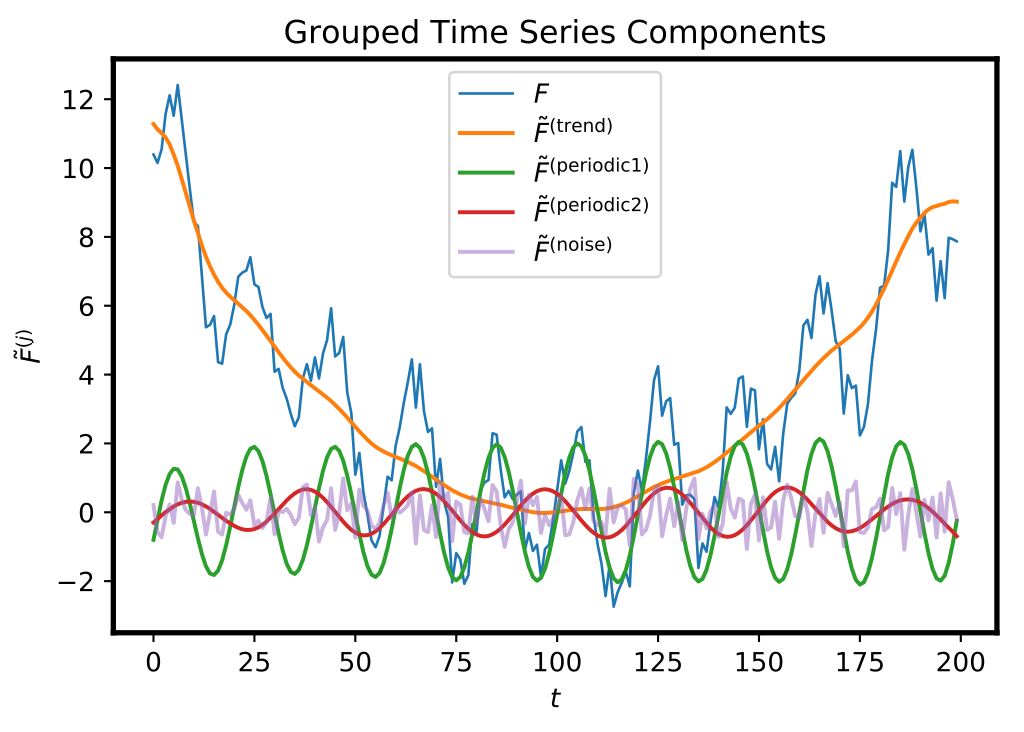
\includegraphics[width=1\textwidth]{Step 1/Singular_spectrum_analysis_grouped_reconstruction}      
\end{column}
\end{columns}
\end{frame}
\end{document}